\documentclass[conference]{IEEEtran}
\IEEEoverridecommandlockouts
% The preceding line is only needed to identify funding in the first footnote. If that is unneeded, please comment it out.
\usepackage{cite}
\usepackage{amsmath,amssymb,amsfonts}
\usepackage{algorithmic}
\usepackage{graphicx}
\usepackage{textcomp}
\usepackage{xcolor}
\usepackage{enumitem}
\def\BibTeX{{\rm B\kern-.05em{\sc i\kern-.025em b}\kern-.08em
		T\kern-.1667em\lower.7ex\hbox{E}\kern-.125emX}}
\bibliographystyle{plain}
\begin{document}
	
	\title{Analisis Perbandingan Performa Pola Arsitektur MVC dan MVVM dalam Mengeksekusi Operasi\\
		{\footnotesize \textsuperscript{}}
		\thanks{}
	}
	
	\author{\IEEEauthorblockN{Andrew Kurniawan Gianto}
		\IEEEauthorblockA{\textit{Informatika} \\
			\textit{Pradita University}\\
			Tangerang, Indonesia \\
			andrew.kurniawan@student.pradita.ac.id}
		\and
		\IEEEauthorblockN{Ryo Ferdinand}
		\IEEEauthorblockA{\textit{Informatika} \\
			\textit{Pradita University}\\
			Tangerang, Indonesia \\
			ryo.ferdinand@student.pradita.ac.id}
		\and
		\IEEEauthorblockN{Eka Rifail Saipuddin Rachman}
		\IEEEauthorblockA{\textit{Informatika} \\
			\textit{Pradita University}\\
			Tangerang, Indonesia \\
			eka.rifail@student.pradita.ac.id}
		\and
		\and
		\and
		\IEEEauthorblockN{Verrel Novendra Sulu}
		\IEEEauthorblockA{\textit{Informatika} \\
			\textit{Pradita University}\\
			Tangerang, Indonesia \\
			verrel.novendra@student.pradita.ac.id}
		\and
		\and
		\and
		\and
		\and
		\and
		\IEEEauthorblockN{Hezel Anthonie Norman Piter Papia}
		\IEEEauthorblockA{\textit{Informatika} \\
			\textit{Pradita University}\\
			Tangerang, Indonesia \\
			hezel.anthonie@student.pradita.ac.id}
	}
	
	\maketitle
	
	\begin{abstract}
		Abstrak akan diisi setelah makalah sudah lengkap dengan pendahuluan, kajian terkait, metodologi, hasil dan pembahasan, serta kesimpulannya.
	\end{abstract}
	
	\begin{IEEEkeywords}
		MVC, MVVM, kecepatan, memori
	\end{IEEEkeywords}
	
	\section{Pendahuluan}
	Perangkat lunak telah menjadi dasar bagi banyak aplikasi dan sistem yang digunakan dalam berbagai hal dalam era teknologi informasi yang terus berkembang. Karena itu, perangkat lunak dibangun agar tidak hanya beroperasi dengan efisien, tetapi juga dapat berkembang dan berubah. Pengembang harus mengatur kode mereka sehingga mudah dipahami dan diselesaikan karena sistem yang kompleks dan masalah berulang. Pola desain antarmuka pengguna dapat membantu mengurangi kekacauan sistem yang kompleks. Penggunaan pola ini akan membuat aplikasi lebih terorganisir dan dapat diskalakan, sehingga tidak terelakkan untuk mempelajari pola antarmuka pengguna dan membuat keputusan yang tepat tentang pola mana yang paling cocok\cite{Perbandingan4}. \textit{Model-View-Controller} (MVC) dan \textit{Model-View-ViewModel} (MVVM) adalah dua arsitektur yang akan dibahas dalam artikel ini.
	
	Tujuan dari penelitian ini adalah untuk membandingkan kinerja arsitektur MVC dengan MVVM, khususnya dalam hal kecepatan dan penggunaan memori. MVC telah menjadi arsitektur yang paling umum digunakan dalam pengembangan perangkat lunak dengan metode prototype, sedangkan MVVM adalah arsitektur yang paling umum digunakan dalam pengembangan aplikasi mobile \cite{Perbandingan4}. Penelitian akan menentukan arsitektur mana yang paling efisien dan paling sesuai dengan berbagai kebutuhan pengembangan perangkat lunak melalui eksperimen untuk masing-masing \textit{Model-View} (MV). 
	
	Penelitian ini diharapkan dapat membantu pengembang perangkat lunak memahami kelebihan dan kelemahan arsitektur melalui eksperimen yang dapat memberikan pemahaman yang lebih baik. Dengan demikian, pengembang dapat memperoleh informasi yang lebih baik dan membuat keputusan yang lebih baik dalam memilih arsitektur yang tepat untuk proyek mereka, sehingga menghasilkan aplikasi yang lebih baik, efisien, dan dapat diandalkan.
	
	
	\section{Kajian Terkait}
	
	\subsection{Model-View-Controller (MVC)}
	\textit{Model-View-Controller} atau MVC adalah arsitektur perangkat lunak untuk membuat sebuah aplikasi dengan memisahkan data (\textit{Model}) dari tampilan (\textit{View}) dan cara bagaimana memprosesnya (\textit{Controller})\cite{Perbandingan4} \cite{MVC} . MVC menekankan tiga elemen penting: perhatian, tanggung jawab, dan logika. Ini mempercepat kinerjanya.
	
	Berikut adalah penjelasan dari masing-masing komponen (Diilustrasikan pada figure 1):
	\begin{enumerate}[label=\alph*]
		\item Bagian \textit{model} biasanya digunakan untuk mengambil data dari database atau menyimpan data ke dalam database. 
		\item Bagian \textit{view} adalah komponen yang menampilkan antarmuka pengguna aplikasi, yang dibangun berdasarkan data model. 
		\item Bagian \textit{control} adalah bagian yang menangani interaksi pengguna, bekerja dengan model, dan menyimpan data ke dalam database.
	\end{enumerate}
	
	\vspace{4.5\baselineskip} 
	
	\begin{figure}
		\centering
		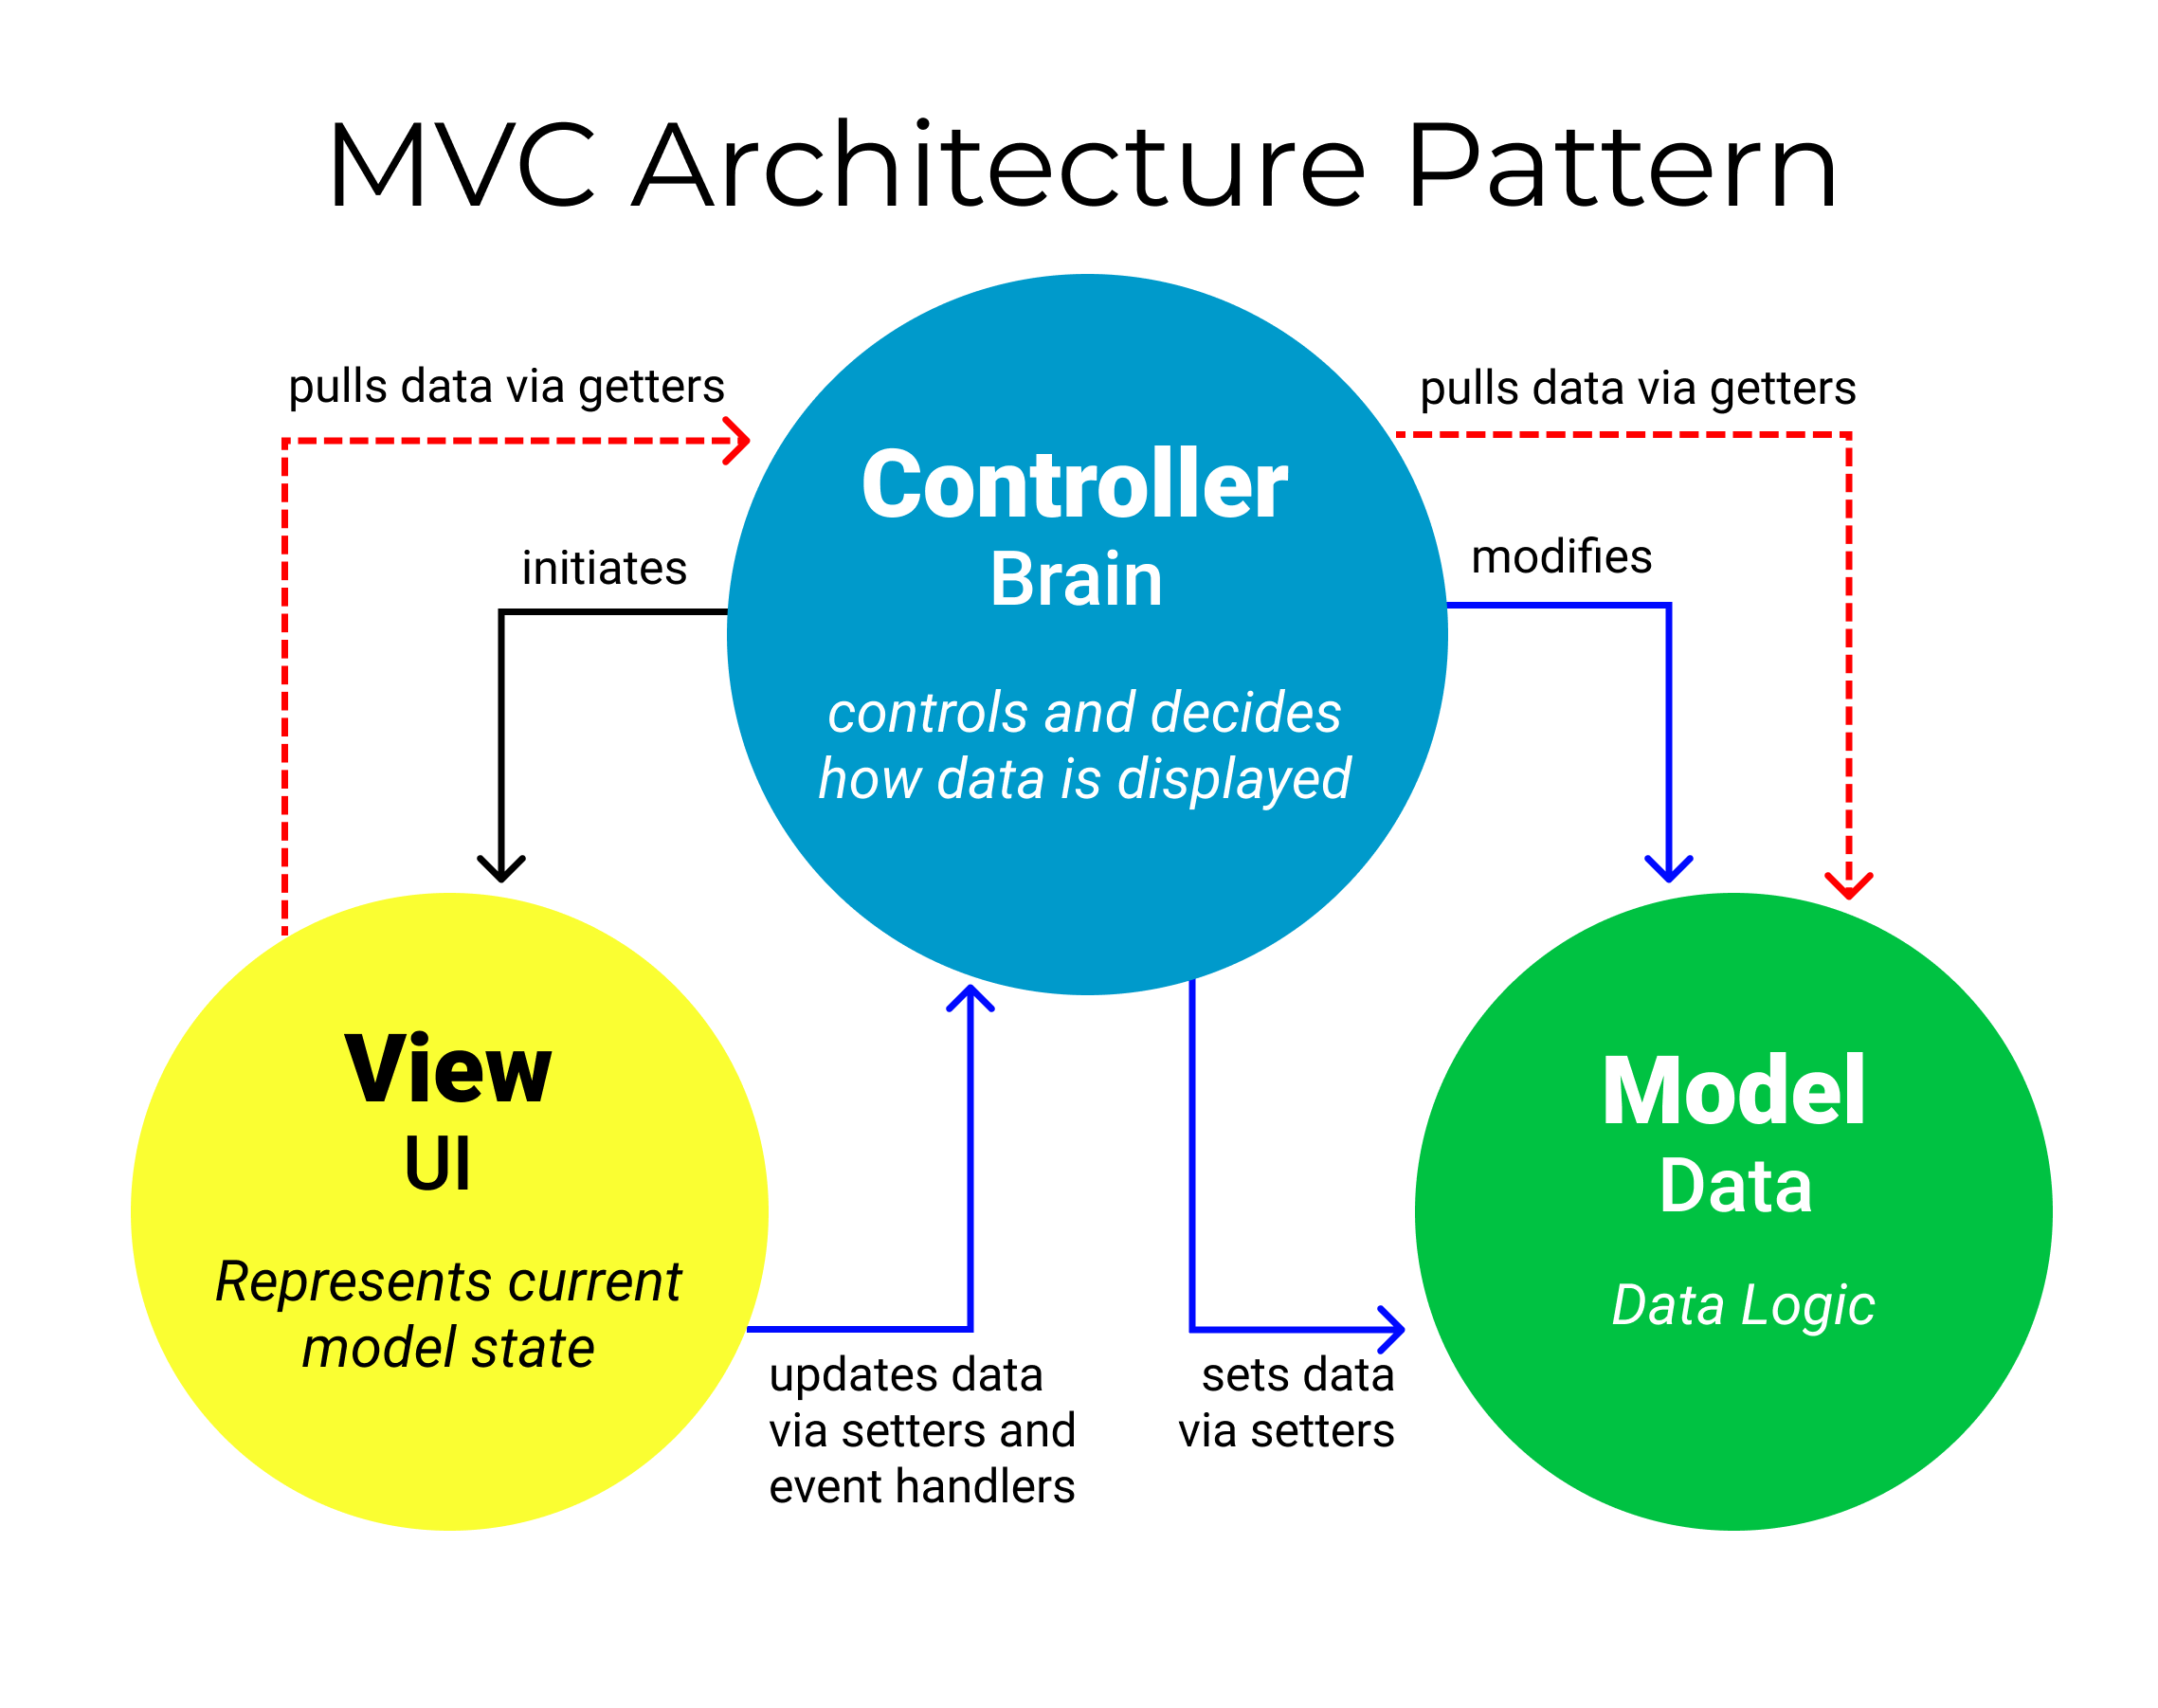
\includegraphics[width=0.5\textwidth]{images/MVC3}
		\caption{Arsitektur MVC}
	\end{figure}
	
	Berikut dijelaskan mengenai keuntungan dan kerugian dari arsitektur MVC:
	\subsubsection{Keuntungan}
	\begin{itemize}
		\item Pemisahan tanggung jawab antara \textit{Model, View,} dan \textit{Control} membuat aplikasi lebih mudah dipahami, diuji, dan dikembangkan.
		\item Fleksibilitas dalam mengganti atau memodifikasi salah satu komponen tanpa memengaruhi komponen lainnya.
		\item Memungkinkan pengembangan paralel antara komponen-komponen aplikasi.
	\end{itemize}
	\subsubsection{Kerugian}
	\begin{itemize}
		\item Adanya kompleksitas dalam pengelolaan koneksi antara 3 komponen tersebut.
		\item Adanya kesulitan dalam pengujian unit pada \textit{View} dan \textit{Controller}.
	\end{itemize}
	
	\subsection{Model-View-View-Model (MVVM)}
	\textit{Model View ViewModel} (MVVM) adalah sebuah arsitektur perangkat lunak yang memisahkan antara kode untuk logika bisnis dan tampilan aplikasi\cite{MVVM}. Dalam kata lain, MVVM adalah sebuah pattern desain yang terdiri dari tiga komponen: \textit{Model, View, dan ViewModel} \cite{MVVM2}.  
	
	Berikut adalah penjelasan dari masing-masing komponen (Diilustrasikan pada figure 2):
	\begin{enumerate}[label=\alph*]
		\item Bagian \textit{model} merupakan representasi dari data yang digunakan dalam logika bisnis.
		\item Bagian \textit{view} adalah komponen yang terdiri dari layout sumber daya file dan aktivitas/fragmen. Activity/Fragment secara dinamis mengontrol tampilan pada layout sumber daya file.
		\item Bagian \textit{ViewModel} berinteraksi dengan Model dan menyiapkan variabel yang akan diamati oleh \textit{View}. \textit{ViewModel} bersifat lifecycle-aware, sehingga kelas ini akan hidup ketika sebuah kelas View telah melalui tahapan create dan belum melalui tahapan destroy.
	\end{enumerate}
	
	
	\begin{figure}
		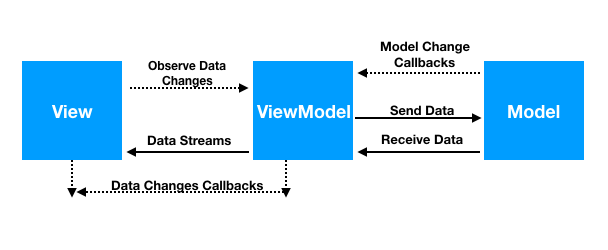
\includegraphics[width=0.5\textwidth]{images/MVVM}
		\caption{Arsitektur MVVM}
	\end{figure}

	Berikut dijelaskan mengenai keuntungan dan kerugian dari arsitektur MVVM:
	\subsubsection{Keuntungan}
	\begin{itemize}
		\item Pemisahan antara \textit{View} dan \textit{ViewModel} sehingga membuat pengujian dan pemeliharaan kode lebih mudah
		\item Kode MVVM biasanya digerakkan oleh peristiwa, yang berarti kode dapat diuji secara terpisah.
	\end{itemize}
	\subsubsection{Kerugian}
	\begin{itemize}
		\item Komponen antarmuka MVVM harus dibuat observable yang berarti dapat memakan waktu dan rumit.
		\item Banyak kode yang harus ditulis dan dikelola untuk setiap komponen UI sehingga aplikasi dapat menjadi lebih sulit untuk digunakan dan dipahami.
	\end{itemize}
	
	\subsection{Perbandingan MVC dan MVVM}
	Dalam penelitian "Perbandingan Kinerja Pola Perancangan MVC, MVP, dan MVVM Pada Aplikasi Berbasis Android (Studi Kasus: Aplikasi Laporan Hasil Belajar Siswa SMA BSS)"\cite{Perbandingan1}, dibahas analisis perbandingan tiga pola perancangan arsitektur perangkat lunak yang populer: Model-View-Controller, Model-View-Presenter, dan Model-View-ViewModel (MVVM).  Aplikasi laporan hasil belajar siswa SMA Brawijaya Smart School digunakan sebagai basis untuk penelitian ini. Tujuan dari penelitian ini adalah untuk menemukan pola perancangan yang paling hemat energi dan memori untuk aplikasi Android. Penelitian dimulai dengan rekayasa untuk menentukan persyaratan fungsional dan non-fungsional. Persyaratan ini kemudian digunakan sebagai dasar untuk desain dan pelaksanaan penelitian. Ketiga pola desain ini digunakan untuk memulai implementasi Java. Setelah tahap implementasi, setiap aplikasi yang menggunakan pola ini diuji. Pengujian dilakukan sebanyak lima kali untuk mendapatkan data penggunaan energi dan memori. Hasil pengujian menunjukkan bahwa ketiga pola perancangan memiliki penggunaan energi yang sederhana, dengan penggunaan memori rata-rata 59,7 MB untuk MVC, 59 MB untuk MVP, dan 73,2 MB untuk MVVM. Selain itu, tahap pengujian fungsional dengan metode pengujian blackbox memberikan hasil validitas sebesar 100\% untuk semua fungsi.
	
	Dalam penelitian "A Comparison of Android Native App Architecture—MVC, MVP, and MVVM"\cite{Perbandingan2}, dibahas mengenai masalah efisiensi dan kualitas pengembangan aplikasi Android yang dipengaruhi oleh arsitektur aplikasi. Tujuan dari artikel ini adalah untuk memberikan analisis menyeluruh untuk menentukan apakah arsitektur MVP (Model-View-Presenter) dan MVVM (Model-View-ViewModel) lebih unggul dari arsitektur aplikasi Android native bawaan, yaitu MVC (Model-View-Controller). Dengan menggunakan Metode Analisis Tradeoff Arsitektur untuk menjawab pertanyaan ini dan menetapkan tiga kriteria: ketepatan, modifikasi, dan kinerja. Berdasarkan kriteria ini, mereka mengenali faktor-faktor penting untuk setiap atribut kualitas dan melakukan perbandingan. Hasil analisis dan eksperimen menunjukkan bahwa MVP dan MVVM lebih unggul daripada MVC dalam hal testability, modifiability (tingkat coupling yang rendah), dan performance (mengonsumsi memori yang lebih sedikit).
	
	Dalam penelitian "Performance Comparison of Native Android Application on MVP and MVVM"\cite{[Perbandingan3]}, dibahas analisis komparatif terhadap arsitektur MVP (\textit{Model-View-Presente}r) dan MVVM (\textit{Model-View-ViewModel}) dalam konteks pengembangan aplikasi Android asli dilakukan dalam makalah yang ditulis oleh Wisnuadhi, Munawar, dan Wahyu. Tujuan dari penelitian ini adalah untuk mengevaluasi kinerja kedua arsitektur tersebut dengan mempertimbangkan tiga faktor: penggunaan CPU, penggunaan memori, dan waktu eksekusi. Hasil eksperimen menunjukkan bahwa arsitektur MVVM lebih baik dalam penggunaan CPU dan waktu eksekusi, sedangkan MVP unggul dalam penggunaan memori. Aplikasi MVVM memiliki penggunaan CPU yang lebih rendah dengan perbedaan rata-rata 0,55\% dan waktu eksekusi yang lebih cepat dengan perbedaan rata-rata 126.21 ms. Aplikasi MVP juga memiliki penggunaan memori yang lebih rendah dengan perbedaan rata-rata 0.92 Mb1.
	
	
	\section{Metodologi}
	
	
	\section{Hasil dan Pembahasan}
	
	
	\section{Kesimpulan}
	
	
	\bibliography{reference.bib}
	\vspace{12pt}
	
\end{document}
